\documentclass{report}
\usepackage{tocloft}
\usepackage{geometry}
\usepackage{graphicx}
\usepackage{caption}
\usepackage[T1]{fontenc}
\usepackage[utf8]{inputenc}
\usepackage[polish]{babel}
\usepackage{float}
\usepackage{listings}
\usepackage{xcolor}

\geometry{
    a4paper,
    left=2.5cm,
    right=2.5cm,
    top=2.5cm,
    bottom=2.5cm,
}

\lstset{
    language=Matlab,
    basicstyle=\footnotesize\ttfamily,
    keywordstyle=\color{blue},
    commentstyle=\color{green},
    stringstyle=\color{red},
    numbers=left,
    numberstyle=\tiny\color{gray},
    stepnumber=1,
    numbersep=5pt,
    backgroundcolor=\color{lightgray},
    frame=single,
    tabsize=2,
    captionpos=b,
    breaklines=true
}


\setcounter{tocdepth}{3}
\setlength{\cftbeforechapskip}{15pt} 
\setlength{\cftbeforesecskip}{8pt} 
\setlength{\cftbeforesubsecskip}{5pt} 
\setlength{\cftbeforesubsubsecskip}{5pt}

\renewcommand\thesection{\arabic{section}.}
\renewcommand\thesubsection{\thesection\arabic{subsection}.}
\renewcommand\thesubsubsection{\thesubsection\arabic{subsubsection}.}
\setcounter{secnumdepth}{3}


\begin{document}


\begin{titlepage}
    \centering
    \vspace*{1cm}
    \begin{figure}
        \centering 
        \includegraphics[width=0.5\textwidth]{"logo.png"}
    \end{figure}
    \Huge
    Zajęcia Projektowe
    \par
    \textbf{Oprogramowanie Systemów Pomiarowych}
    
    \vspace*{1cm}

    \vspace{0.5cm}
    \LARGE \textit{Aplikacja autoryzacji dostępu oparta 
    na biometrycznej weryfikacji tożsamości}
    
    \vspace{1.5cm}
    
    \textbf{Autorzy:} 
    \par
    Jakub Pająk 
    \par
    Łukasz Grabarski
    \par 
    Krzysztof Grądek
    \par 
    Piotr Legień
    \vspace*{1.5cm}
    \par AiR Grupa 5TI
    
    \vfill
    
    \Large 16.05.2024
    
\end{titlepage}


\newpage

\tableofcontents

\newpage


\section{\LARGE Wprowadzenie}
\subsection{\Large Cel projektu}
Celem projektu była implementacja aplikacji mającej główną część logiki osadzoną w środowisku progtamistycznym 
LabView oraz napisanie skryptu w języku Python realizującego rozpoznawanie twarzy w celu autoryzacji dostępu. 


\subsection{\Large Założenia wstępne}
Wstępne odgórne założenia implikowały wykorzystanie środowiska programistycznego LabView z szczególnym warunkiem jakim było wykorzystanie 
maszyny stanów JKI - jednego z znaczących framework-ów LabView. 

Rdzeń aplikacji winien był być osadzony w wcześniej wymienionej maszynie stanów. 
Kolejnym wymaganiem było napisanie odpowiedniej funkcji w języku Python porównującej pobrane zdjęcie podczas próby logowania z zdjęciami znanych użytkowników.
Ponadto należało zaimplementować prostą bazę danych do zarządzania znanymi użytkownikami oraz ich danymi. 

\subsection{\Large Harmonogram realizacji projektu}
\subsubsection{Okres 1}
Zaprojektowanie podstawowego interfejsu użytkownika w środowisku LabVIEW. Dodanie stosownych pól 
oraz przycisków umożliwiających późniejsze logowanie oraz nawigację po aplikacji.

\subsubsection{Okres 2}
Zapoznanie się z sposobem połączenia oraz wywołania skryptu napisanego w języku Python z poziomu środowiska LabView.
Implementacja podstawowej wersji skryptu zdolnego do poprawnego porówniania dwóch obrazów zawierających twach potencjalnego użytkownika.
Próba wywołania skryptu w aplikacji LabView.

\subsubsection{Okres 3}
Dostosowanie skryptu do odpowiednich folderów oraz zmiana implementacji tak, aby kod sprawdzał czy użytkownik próbujący zalogować się do aplikacji widnieje wśród użytkowników 
znanych, czyt. uprzednio dodanych do folderu.
Zapoznanie się z sposobem połączenia apliakcji LabView z relacyjną bazą danych SQL Server.

\subsubsection{Okres 4}
Wdrożenie połączenia z bazą danych oraz weryfikacja poprawności połączenia przy wykorzystaniu podstawowych operacji takich jak SELECT lub INSERT.
Testy aplikacji.

\section{\LARGE Dokumentacja aplikacji}

\subsection{\Large Zagadnienia ogólne oraz środowiska programistyczne}
Aplikacja została zrealizowana w zaawansowanym środowisku programistycznym produkowanym przez firmę National Instruments, znanym jako LabView. Jest to blokowy język programowania, który umożliwia stosunkowo szybkie tworzenie szerokiej gamy aplikacji. Obszerna paleta dostępnych rozszerzeń oraz dodatkowych pakietów znacząco zwiększa efektywność pracy w języku LabView. Wiele złożonych zagadnień można rozwiązać za pomocą kilku elementów z odpowiednich bibliotek. Jednakże, ze względu na nietypowy sposób tworzenia programów w LabView, okres adaptacji do tego nowego środowiska może być nieco dłuższy.

Drugim środowiskiem programistycznym, które zostało wykorzystane, jest Python w wersji 3.10. Szczegółowe uzasadnienie wyboru tej konkretnej dystrybucji języka zostanie przedstawione w dalszych częściach dokumentacji. Podobnie jak LabView, język Python umożliwia dostęp do szerokiej gamy gotowych rozwiązań, które umożliwiają rozwiązywanie złożonych problemów. W związku z tym, w projekcie zastosowano bibliotekę OpenCV wraz z nowoczesnym pakietem face-recognition. Wykorzystanie tych pakietów sprawiło, że implementacja logiki rozpoznawania twarzy stała się zadaniem prostym i efektywnym.

Trzecim środowiskiem programistycznym, jakie zostało użyte, jest SQL Server w połączeniu z systemem SQL Management Studio (SSMS). Ostatni element aplikacji, polegający na dodaniu bazy danych do środowiska LabView, został zrealizowany przy użyciu tych narzędzi. Proces ten nie był tak prosty, jak mogłoby się wydawać na pierwszy rzut oka, dlatego zostanie dokładnie omówiony w odpowiedniej sekcji dokumentacji.


\subsection{\Large Omówienie szkieletu aplikacji - Framework LabView JKI}

Framework LabView JKI jest zaawansowanym zestawem narzędzi oraz wzorców projektowych stworzonych z myślą o usprawnieniu procesu tworzenia aplikacji w środowisku LabView. Jest on szczególnie ceniony za swoje podejście modularne, które umożliwia tworzenie skalowalnych i łatwych do utrzymania aplikacji.

\subsubsection*{Struktura Frameworka}

Framework LabView JKI charakteryzuje się jasno zdefiniowaną strukturą, która ułatwia organizację kodu. Składa się z modułów, które są niezależnymi jednostkami funkcjonalnymi, co pozwala na efektywną separację zadań i logiki aplikacji. Moduły te mogą być łatwo integrowane i wymieniane, co zapewnia elastyczność w zarządzaniu projektem oraz wprowadzaniu zmian.

\subsubsection*{Zarządzanie zasobami i procesami}

Jednym z kluczowych aspektów frameworka JKI jest jego podejście do zarządzania zasobami i procesami. Wykorzystuje on wzorzec aktorów, gdzie każdy aktor reprezentuje autonomiczną jednostkę wykonawczą odpowiedzialną za konkretne zadania. Komunikacja pomiędzy aktorami odbywa się za pomocą wiadomości, co minimalizuje ryzyko konfliktów i zapewnia płynność operacji.

\subsubsection*{Efektywność i optymalizacja}

Framework JKI zawiera szereg narzędzi wspomagających optymalizację aplikacji. Dzięki wbudowanym mechanizmom monitorowania i debugowania, deweloperzy mogą szybko identyfikować i rozwiązywać problemy wydajnościowe. Ponadto, framework wspiera zarządzanie pamięcią oraz zasobami systemowymi, co jest kluczowe dla utrzymania wysokiej wydajności aplikacji nawet przy intensywnym obciążeniu.

\subsubsection*{Integracja z innymi technologiami}

Framework LabView JKI został zaprojektowany z myślą o łatwej integracji z innymi technologiami i systemami. Obsługuje różnorodne protokoły komunikacyjne oraz standardy wymiany danych, co umożliwia płynne połączenie z zewnętrznymi bazami danych, urządzeniami pomiarowymi oraz innymi aplikacjami. Dzięki temu, możliwe jest tworzenie kompleksowych rozwiązań, które są w stanie sprostać najbardziej wymagającym zadaniom.

\subsubsection*{Dokumentacja i wsparcie społeczności}

Framework JKI jest dobrze udokumentowany, co znacznie ułatwia naukę i wdrażanie jego elementów w projekcie. Obszerna dokumentacja zawiera szczegółowe opisy funkcji, przykłady kodu oraz najlepsze praktyki. Dodatkowo, aktywna społeczność użytkowników i deweloperów stanowi cenne źródło wsparcia oraz inspiracji, co jest szczególnie ważne w przypadku napotkania problemów lub wątpliwości.

\subsection{Framework JKI - opis podstawowych stanów}
Sekcja ta ma na celu wprowadzenie użytkownika dla którego programowanie w LabVIEW, a w szczególności z wykorzystaniem framework-a JKI jest obce. 
Framework ten ma pewne elementy specyficzne dla siebie, a których rozumienie jest kluczowe w rozumieniu zasady działania aplikacji. 

Warto nadmienić, że bardzo pomocym narzędziem podczas korzystania z LabView jest Help - można użyć skrótu klawiszowego CTRL + H. 
Informacje zawarte w pomocy są często bardzo pomocne, jeśli nie wystarczają można przejść do linka "Detailed help", tam znajdują się bardzo szczegółowe informacje oraz niekiedy przykłady użycia.
\subsubsection{Ogólny wygląd schematu blokowego JKI}
\begin{figure} [H]
    \centering
    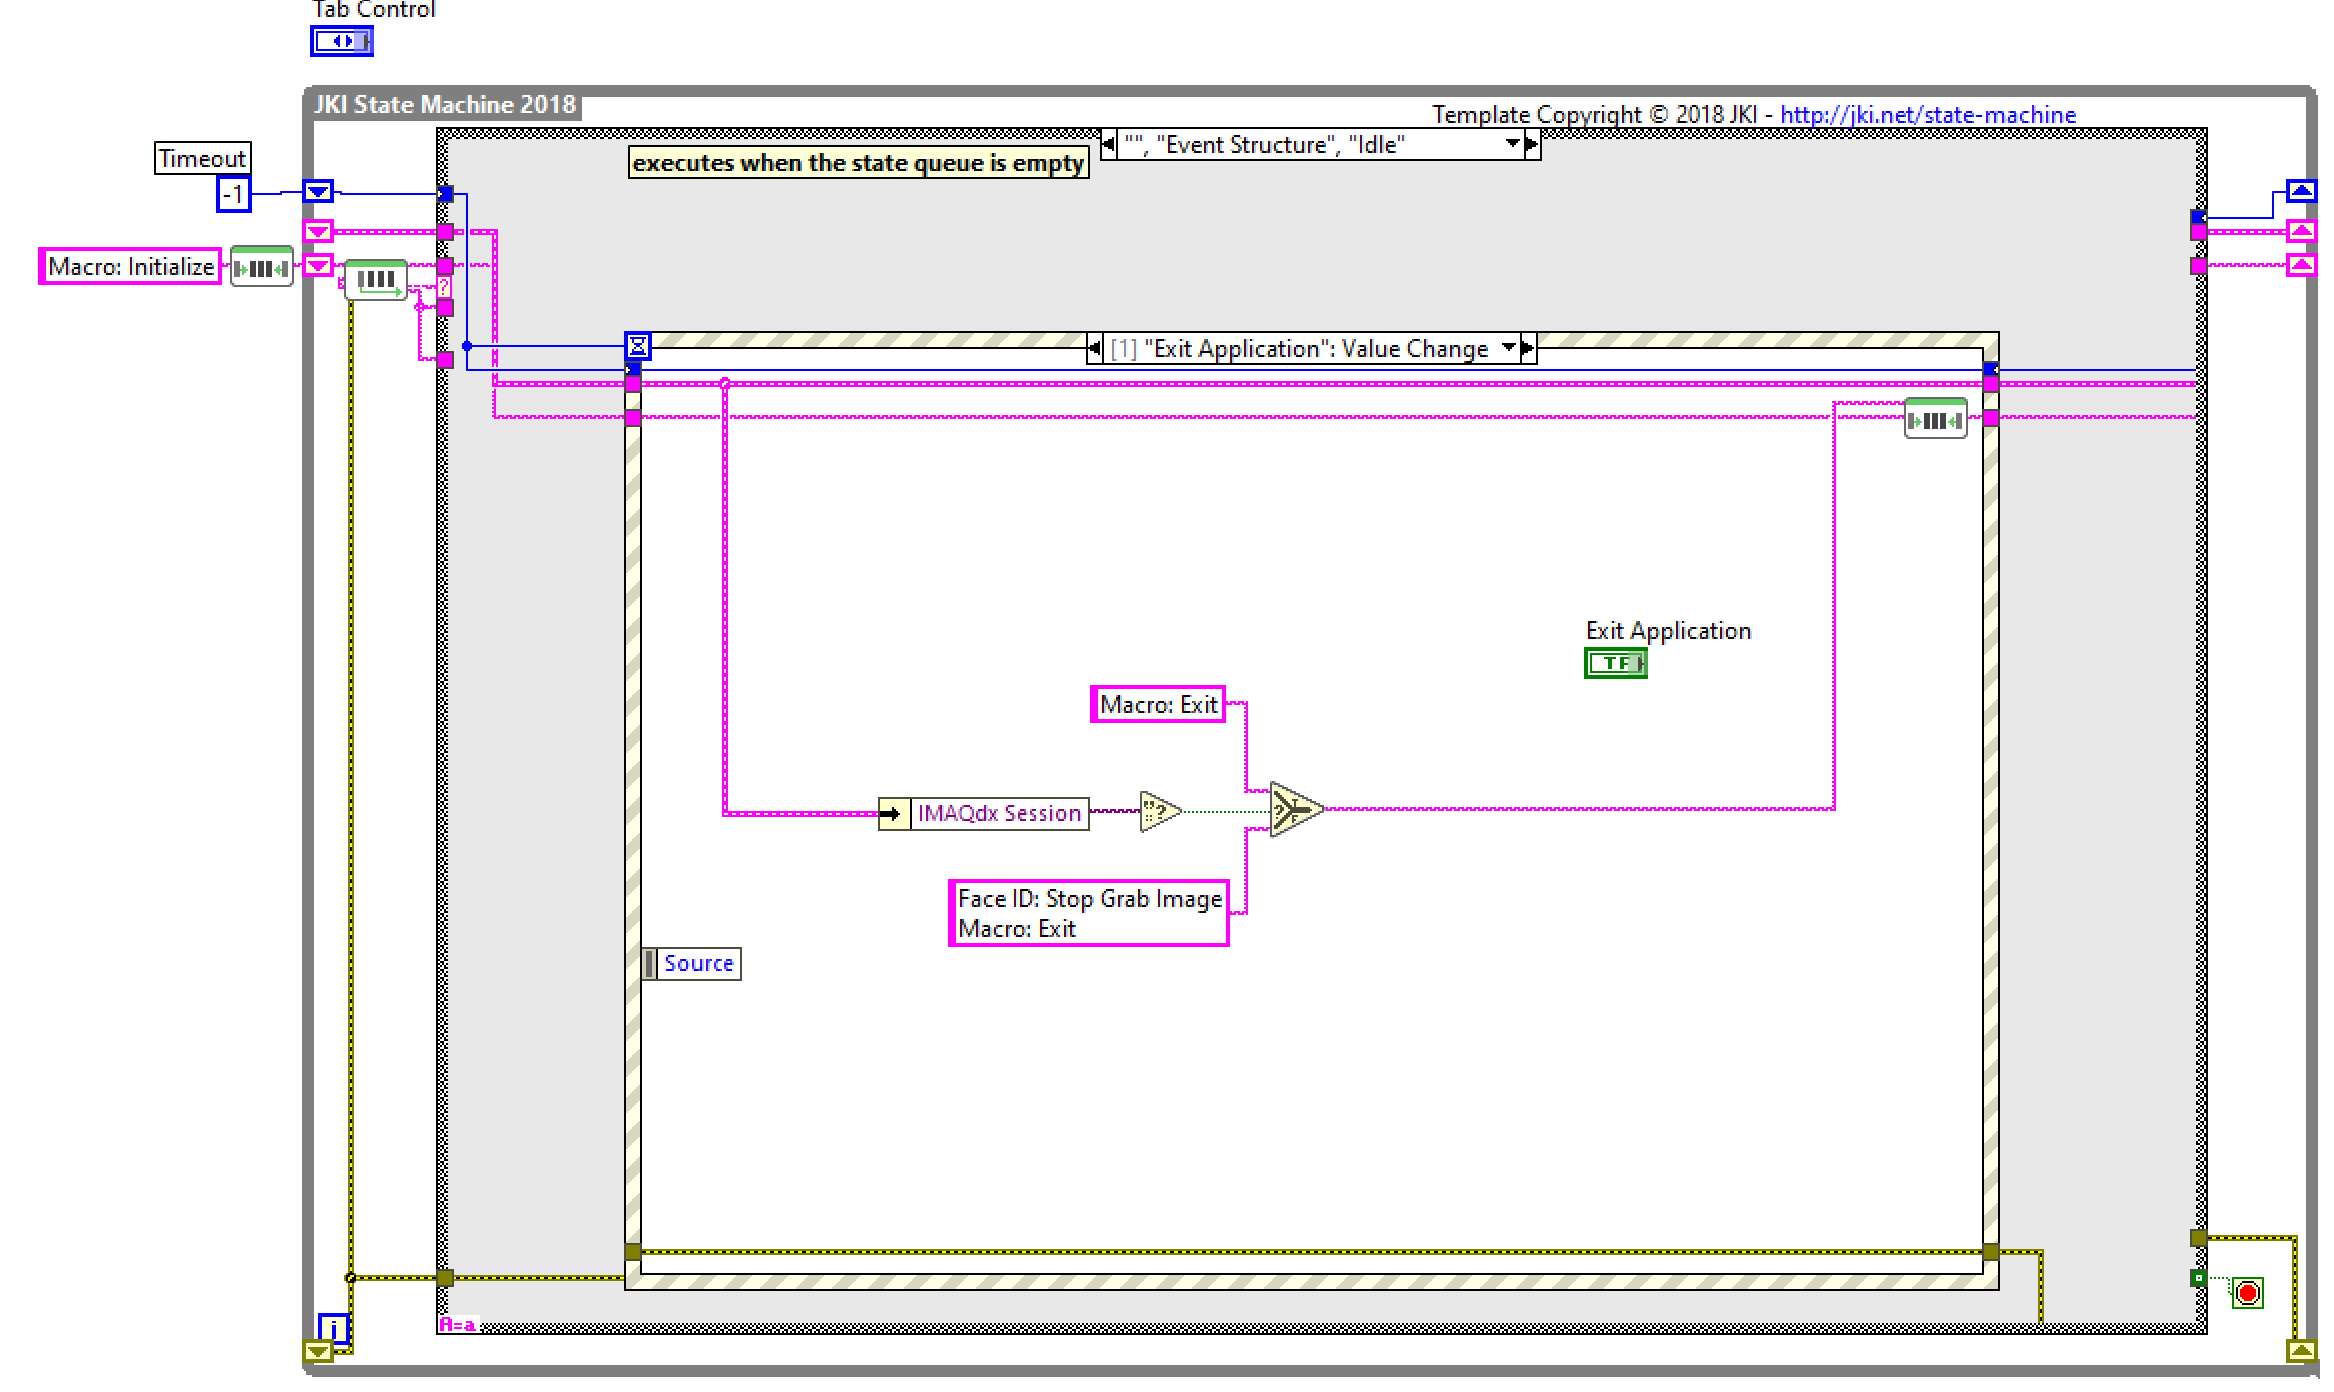
\includegraphics[width=1.0\textwidth]{"src/jki-main.png"}
    \caption{Zdjęcie przedstawiające podstawowy widok schemtu blokowego maszyny stanów JKI}
    \label{fig:foto1}
\end{figure}

Maszyna stanów JKI składa się z dwóch głównych elementów:
\begin{itemize}
    \item Pętli While,
    \item Struktury Case.
\end{itemize}

Pętla while odpowiada za nieskończone (naturalnie do momentu zdarzenia kończącego działania aplikacji) wykonywanie się aplikacji w pętli.
Podczas uruchomienia aplikacja rozpoczyna pracę w pętli oraz przechodzi przez kolejne stany (case) aplikacji.

Drugim elementem jest struktura Case, która odpowiada za naturę działania maszyny stanów - przechodzenie do odpowiednich stanów zdefiniowanych podczas uruchomienia oraz następnie zaciąganych z kolejki. 

\begin{figure} [H]
    \centering
    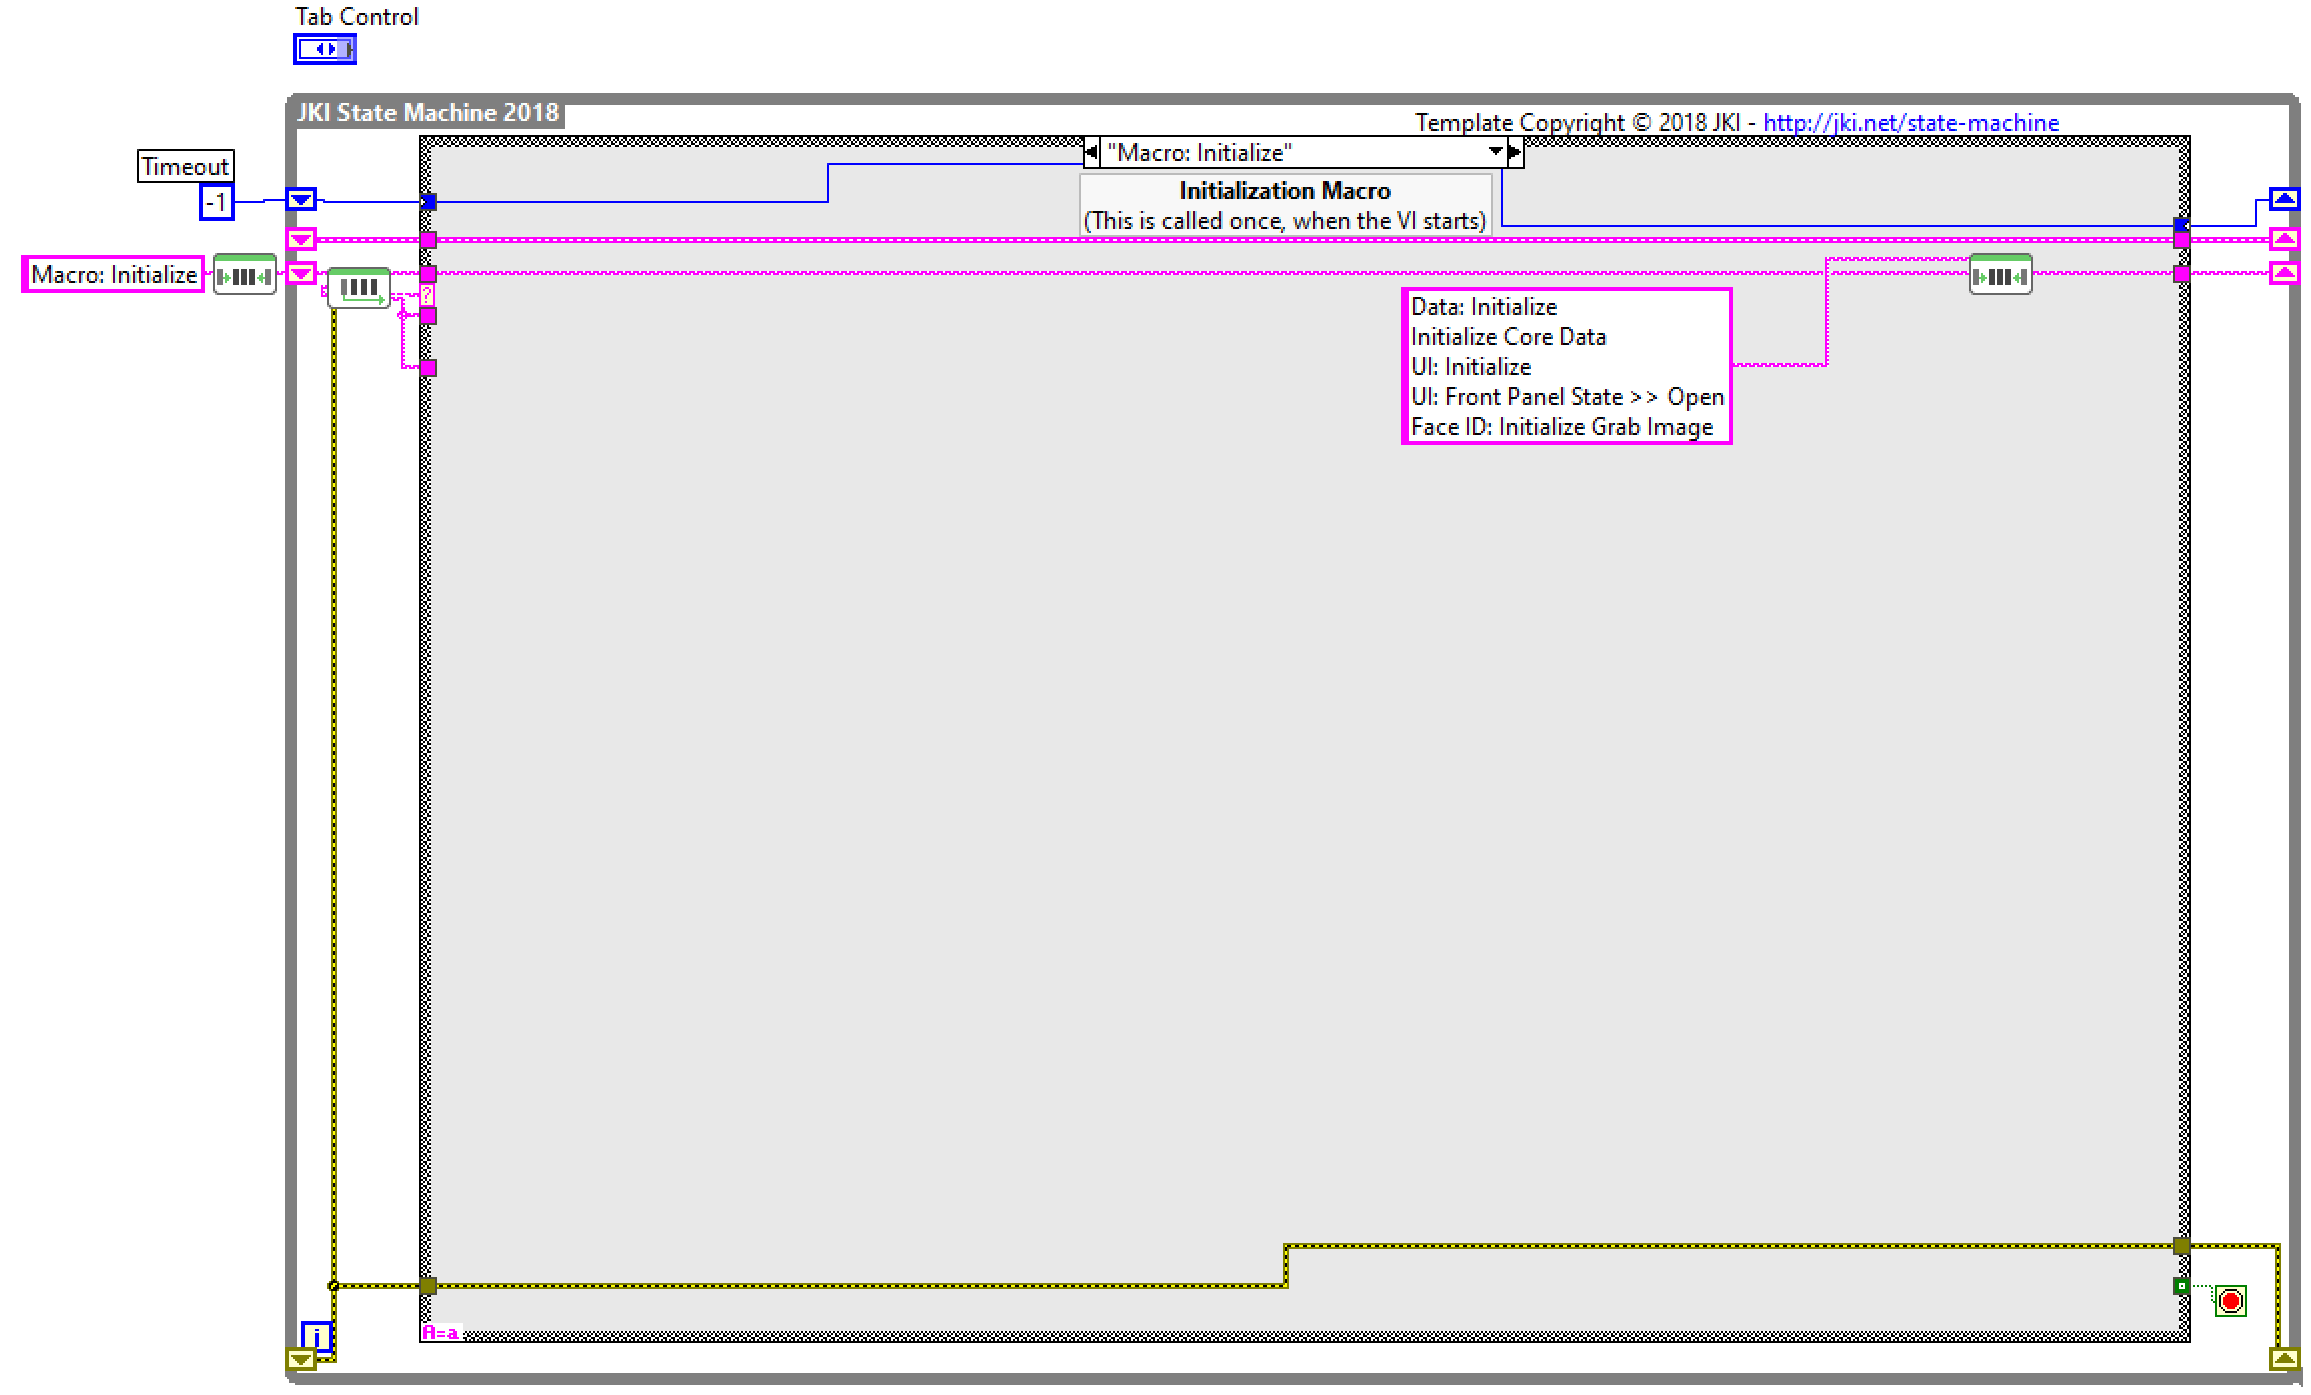
\includegraphics[width=1.0\textwidth]{"src/macro-init.png"}
    \caption{Zdjęcie przedstawiające stan "Macro: Initialize"}
    \label{fig:foto2}
\end{figure}

Stan "Macro: Initialize" jest wykonywany podczas startu aplikacji (jest to wyszczególnione pod rozwijaną listą ze stanami). Ważnym elementem jest pole statyczne typu String (oznaczone typowo kolorem różowym) 
zawierające pięć kolejnych stanów, które zostaną wysłane na kolejkę w celu odpowiedniego toku wykonywania. Najpierw wykona się stan Data: Initialize, następnie Initialize: Core Data etc. 
Na samym końcu zostanie wywołany stan Face ID: Initialize Grab Image. Jest to pierwszy stan, który nie jest zapewniony przez framework, a zatem kod napisany samodzielnie rozpoczyna się wraz z wywołaniem stanu piątego. 

\begin{figure} [H]
    \centering
    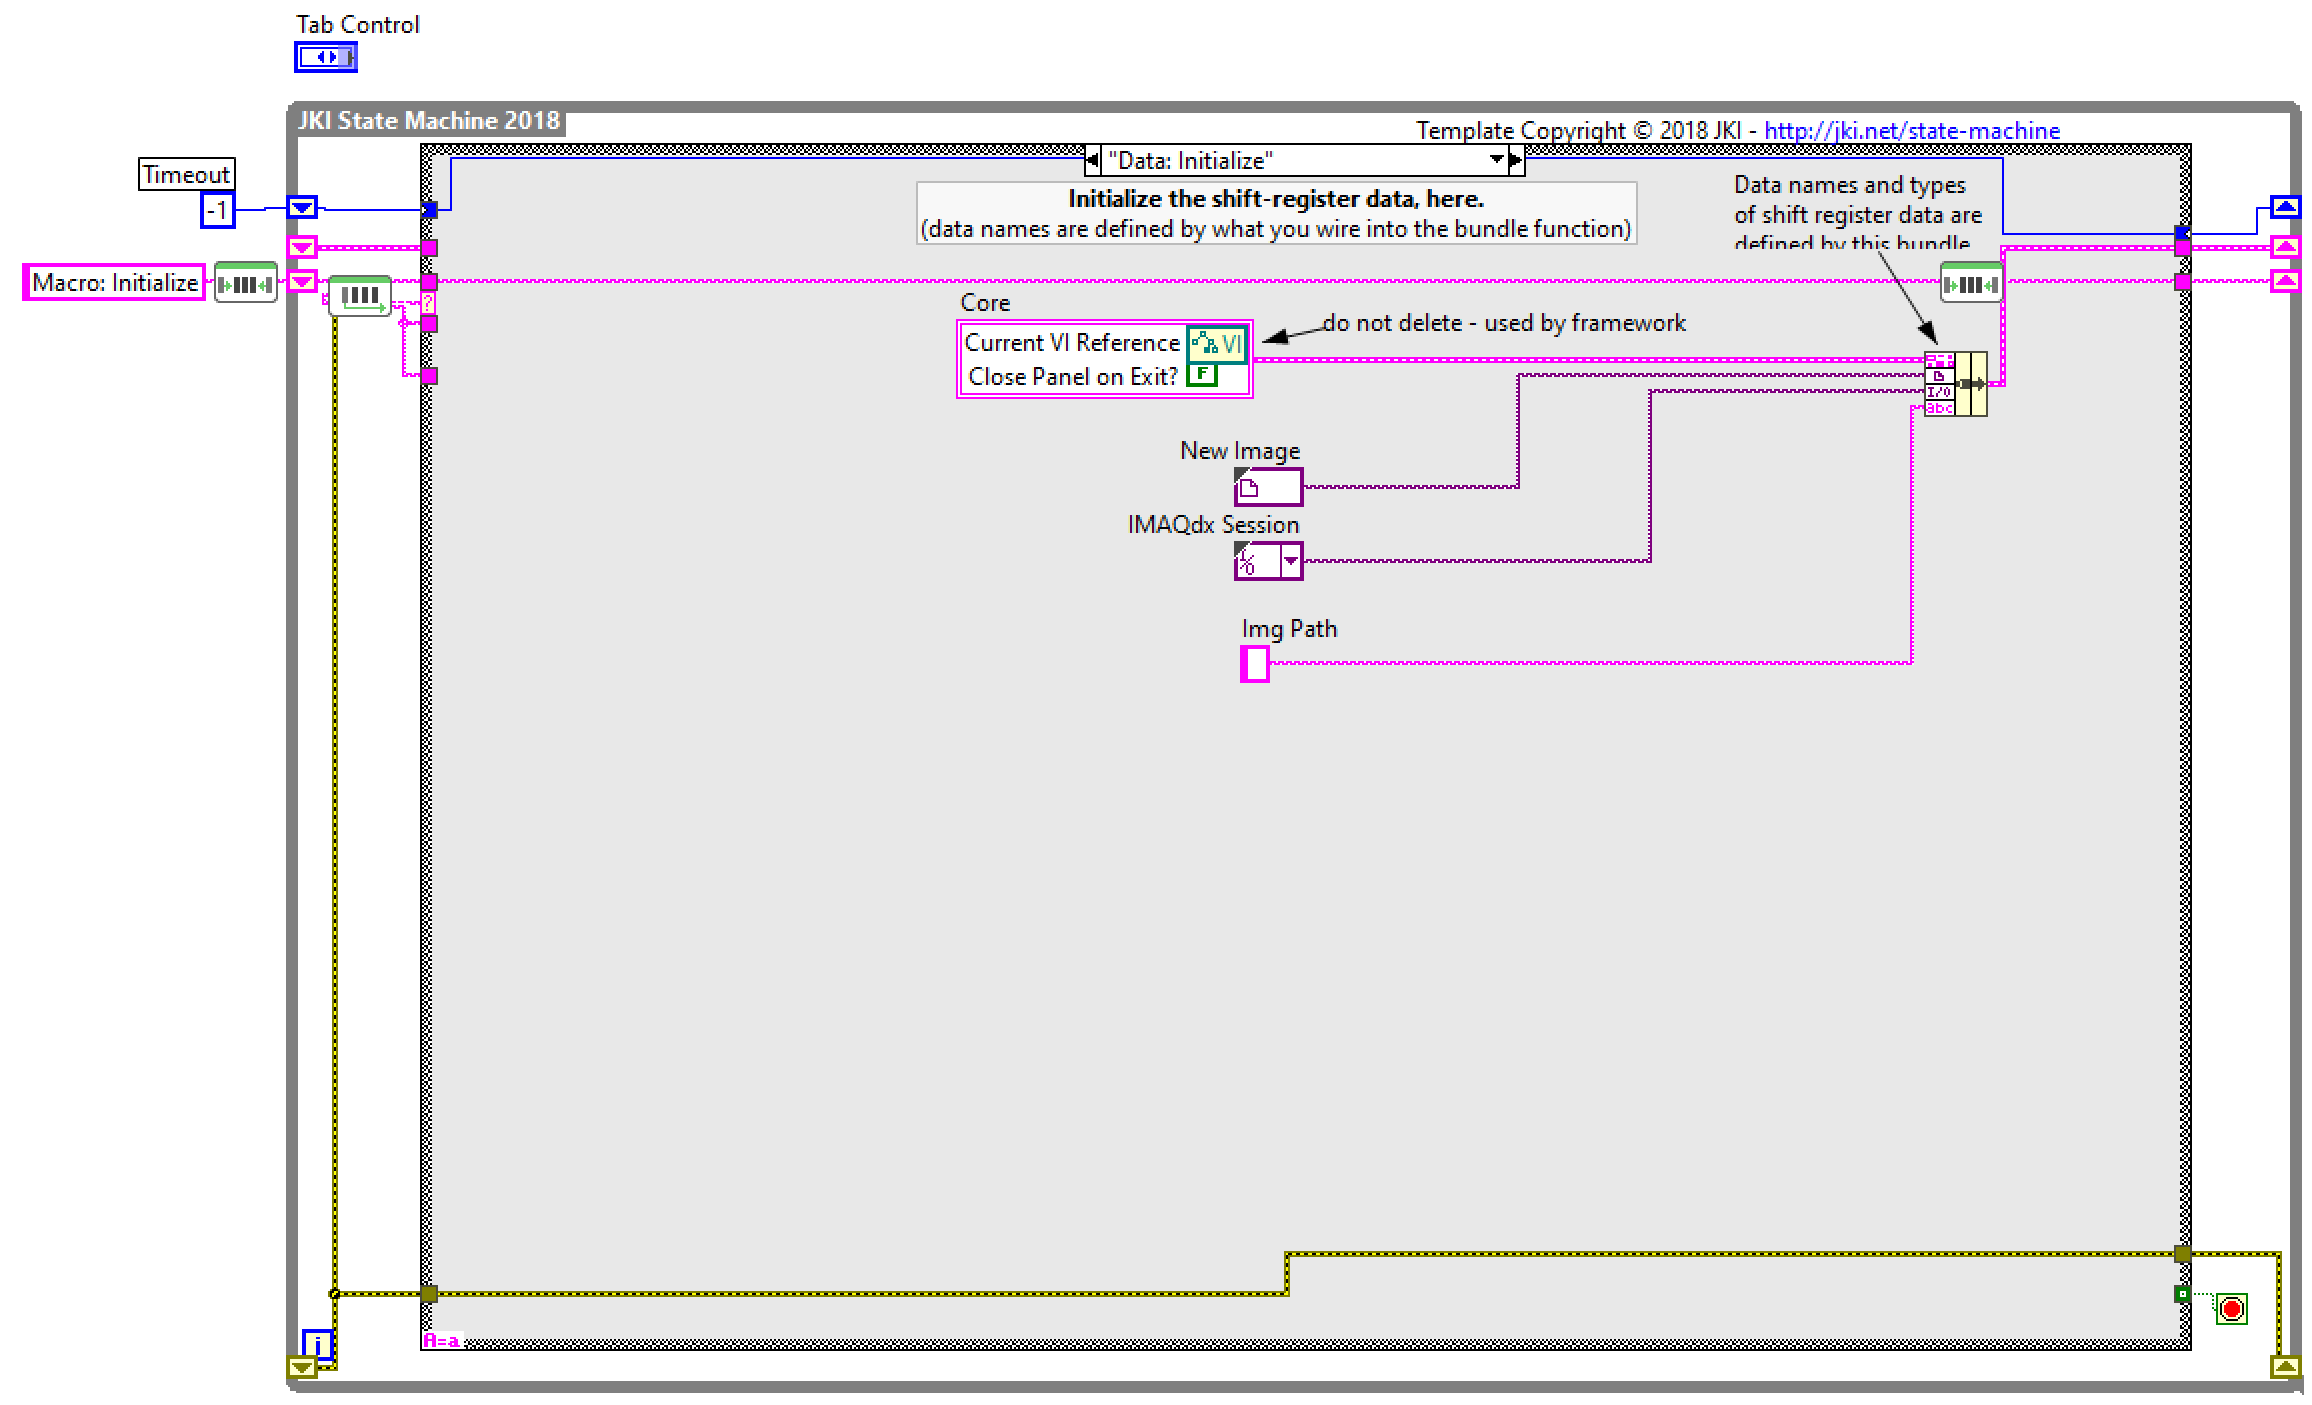
\includegraphics[width=1.0\textwidth]{"src/data-init.png"}
    \caption{Zdjęcie przedstawiające stan "Data: Initialize"}
    \label{fig:foto3}
\end{figure}

Stan "Data: Initialize" odpowiada za inicjalizację żyły zawierającej dane przepływające między stanami. Dzięki wykorzystaniu tej możliwości można przekazywać dowolne dane między kolejnymi stanami oraz modyfikować te dane. 
Dokładne wykorzystanie tej opcji zostanie zaprezentowane w dalszej części dokumentacji. 
Na potrzeby projektu linia danych jest inicjalizowana za pomocą trzech zmiennych:

\begin{itemize}
    \item New Image - przechowuje obraz, jest to zmienna typowa dla biblioteki IMAQ,
    \item IMAQdx Session - kolejna zmienna typowa dla biblioteki IMAQ, przechowuje referencję do otwartek sesji kamery,
    \item Img Path - zmienna typu String przechowująca ściezkę do nowo pobranego zdjęcia.
\end{itemize}

\begin{figure} [H]
    \centering
    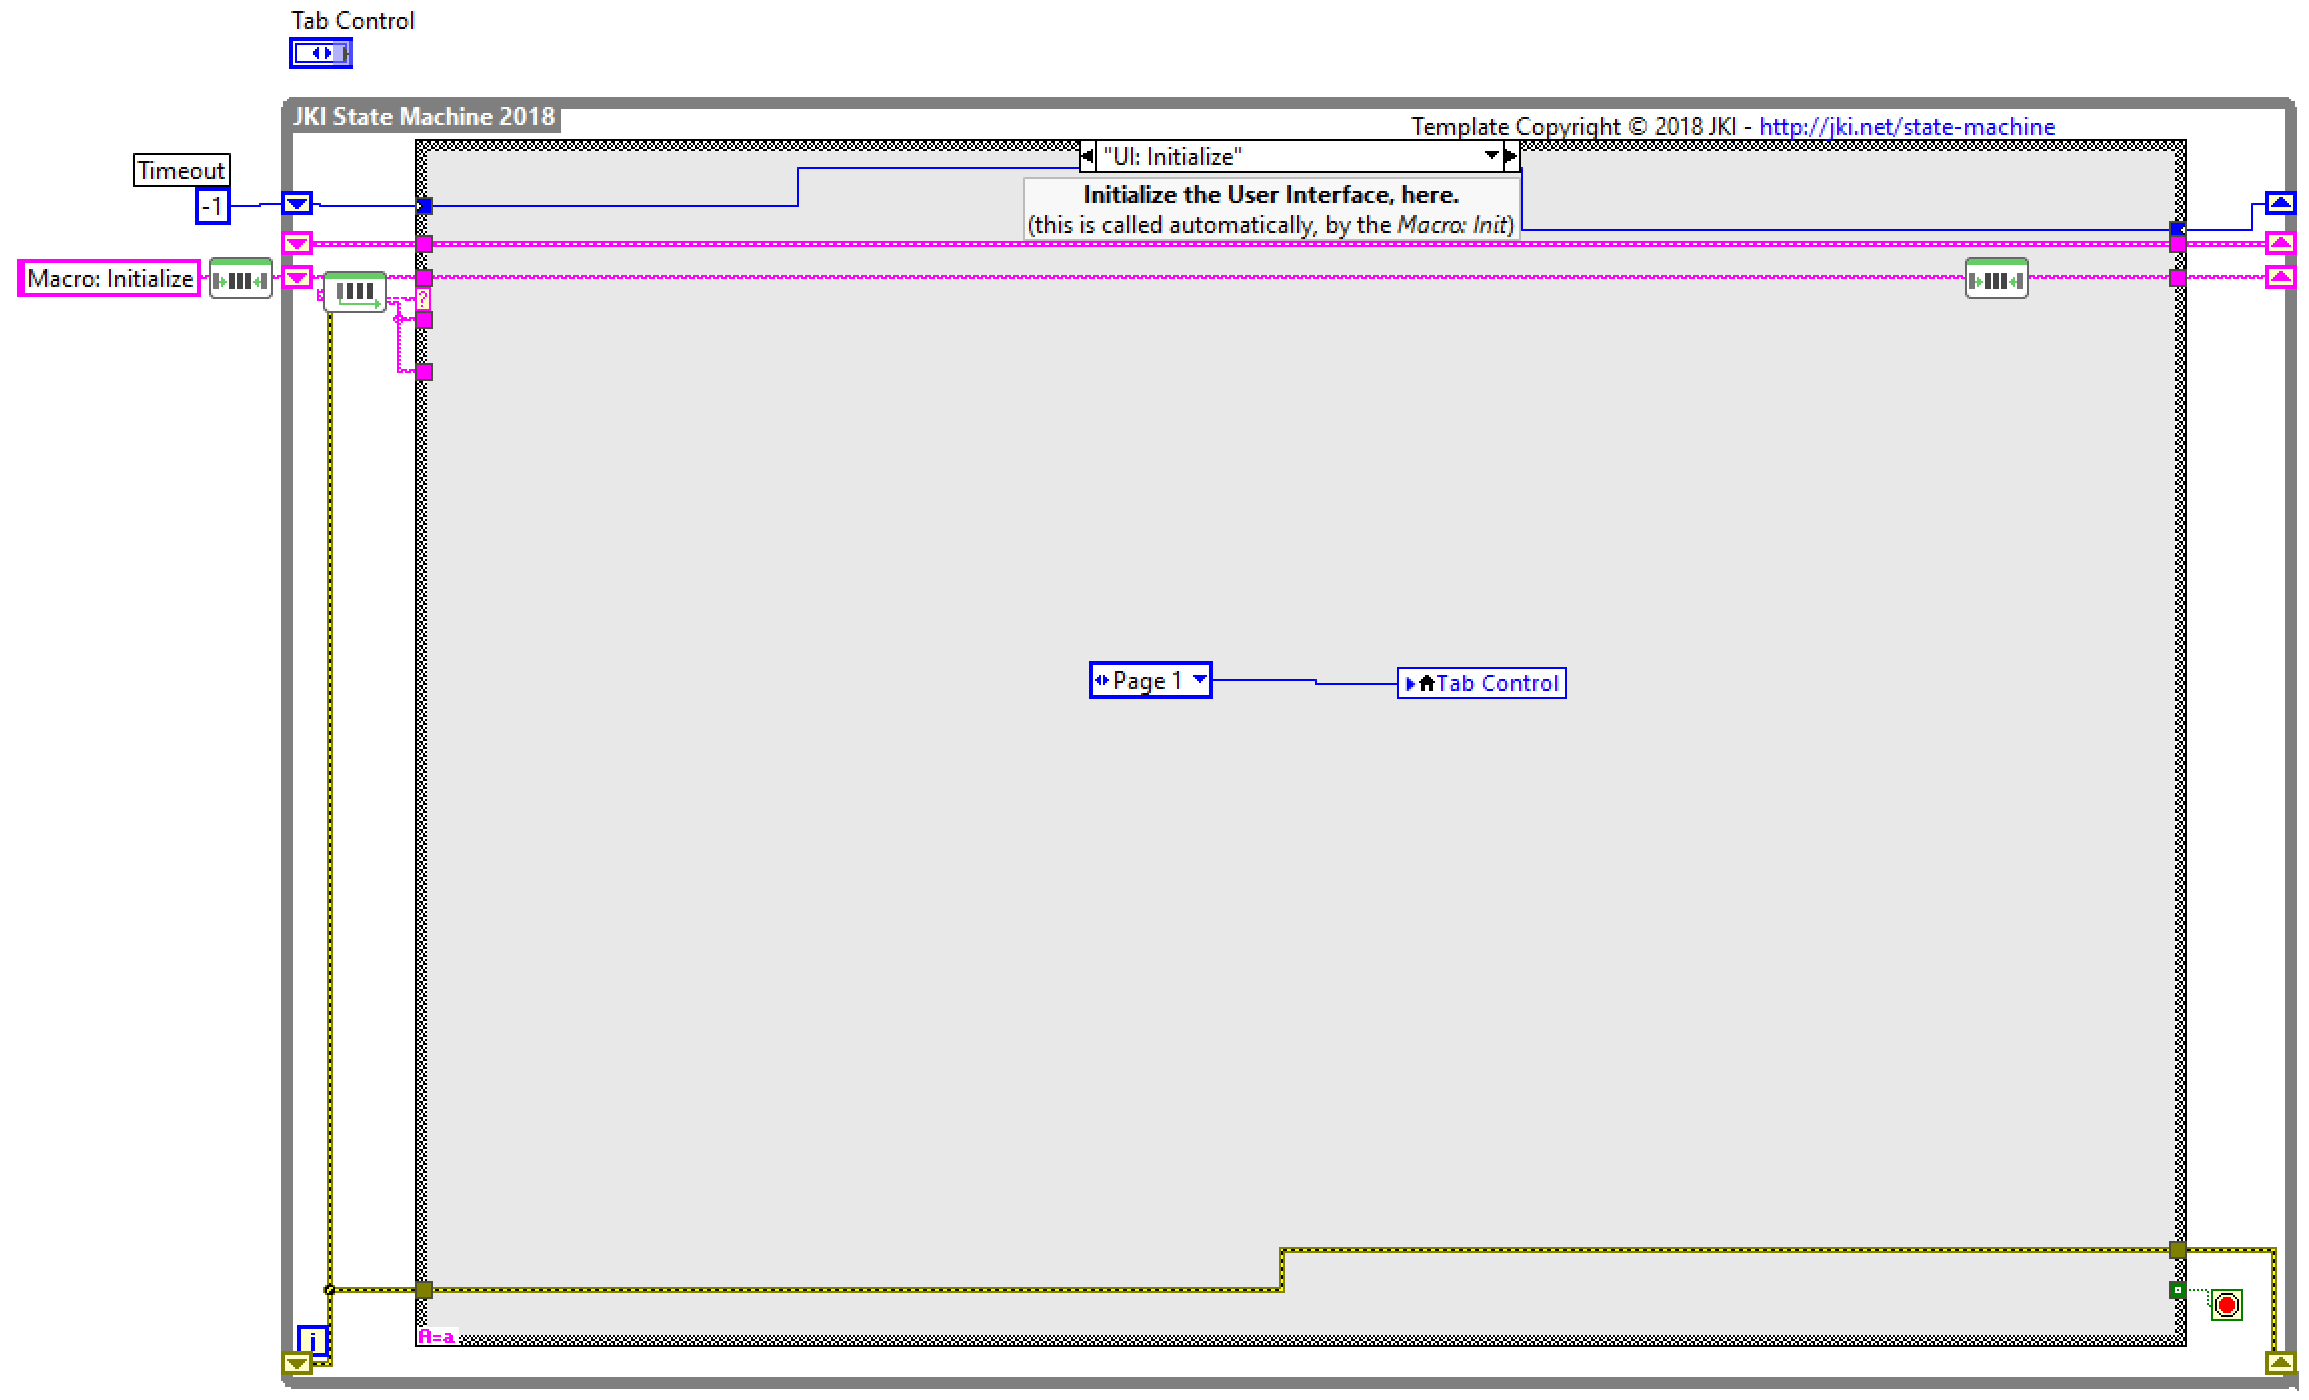
\includegraphics[width=1.0\textwidth]{"src/UI-init.png"}
    \caption{Zdjęcie przedstawiające stan "UI: Initialize"}
    \label{fig:foto4}
\end{figure}

Stan "UI: Initialize" odpowida za wyświetlenie podstawowego widoku aplikacji. W przypadku powyższego projektu odpowiada on za wyświetlenie 
pierwszej zakładki aplikacji przy pomocy struktury Tab dostarczanej przez LabVIEW. 
Element "Page 1" jest standardowym typem wyliczeniowym enum zawierającym deklaracje poszczególnych zakładek. 
Element "Tab Control" odpowiada za wyświetlenie odpowiedniej strony na podstawie wybranej opcji w typie wyliczeniowym.


\subsection{\Large Implementacja procesu logowania w LabView}
Proces logowania jest procesem złożonym z kilku stanów, każdy stan zostanie szczegółowo opisany w poniższej sekcji. 
\subsubsection{\large Stan Face ID: Initialize Grab Image}
Powyższy stan jest odpowiedzialny za inicjalizację kamery w celu późniejszej akwizycji obrazu podczas logowania. 

\subsubsection{\large Stan Face ID: Grab Image}

\subsubsection{\large Stan Face ID: Stop Gram Image}

\subsection{\Large Implementacja identyfikacji użytkownika}

\subsubsection{\large Stan Face ID: Image Processing}

\section{\LARGE Napotkane problemy}
\subsection{\Large Implementacja zakładek}

\subsection{\Large Wywoływanie skryptów Python z poziomu LabVIEW}

\subsection{\Large Wykonanie działającego połączenia aplikacji z bazą danych SQL}

\section{\LARGE Podsumowanie}

\end{document}
